\documentclass[twocolumn]{article}
\usepackage[margin=1in]{geometry}
\usepackage{graphicx}
\graphicspath{ {C:/John/LaTeX/Scioly/Wright Stuff/Trimming/images/} }
\usepackage{grffile}
\usepackage{gensymb}
\usepackage{gensymb}

\title{Trimming in Wright Stuff}
\author{John Yang}
\date{March 19, 2019}

\begin{document}

\twocolumn[
  \begin{@twocolumnfalse}
\maketitle
\begin{abstract}
Here, we will discuss various ways of trimming a model aircraft, specifically relating to Dave Zeigler's Freedom Flight Models kit, \emph{Fun Science 2019 ``Tandem"}.\footnotemark\-\  Use this article, plus the Freedom Flight instructions for guidance. Trimming your airplane becomes the most important thing next to building, and doing this correctly will make or break you. Read this article after the main article. 
\end{abstract}
\end{@twocolumnfalse}
]
\footnotetext{\emph{Adapted from the FS2019 Build Instructions}}

After attaching the stab check the CG of the plane, with the prop and rubber attatched. Hold the plane upside down and use a pencil to find the balance point. The CG should be in the middle of the rubber so you can vary the rubber without messing up the CG. However, in the beginning, start with a CG a half inch forward from the center of the rubber. Of course, you must test, assess, and adjust to find the optimal location. Add bits of clay to adjust the CG location. 

After building your plane, it is recommended to start with 2 grams of .094" rubber. Indeed, .094" rubber is the most widely used and accepted thickness in Wright Stuff. Use 40$\times$15 winds and launch as normal with a $0\degree$ angle of attack. There won't be much torque on it; the purpose is to determine its flight pattern without climbing. Using this amount of torque, the goal is to analyze the effect of the wing angle on the flight pattern. With these settings, the optimal flight path is smooth, level, with a gentle left turn. If the plane nosedives, increase the wing angle of incidence. If it stalls, raise the rear post (don't decrease the front). During cruise, aim for a level motorstick. 

\begin{figure}[h]
\caption{The clich\'e but important picture we always see}
\centering
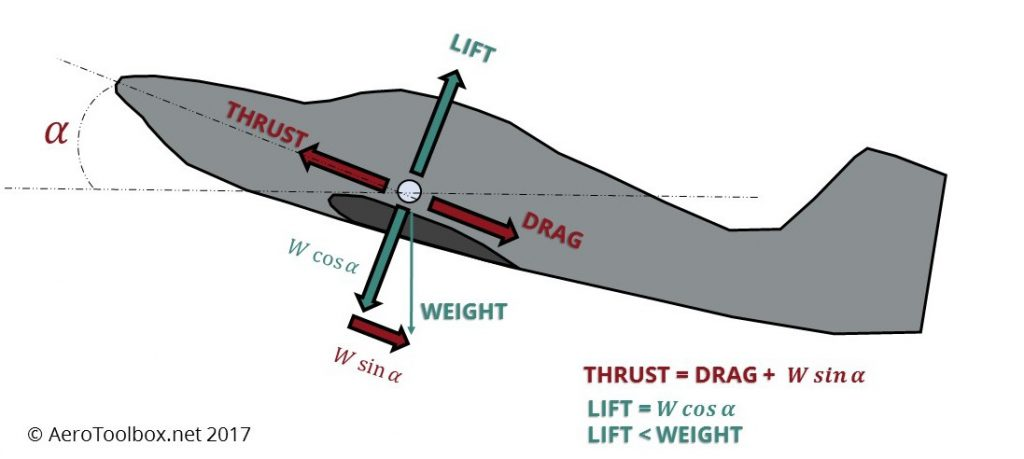
\includegraphics[scale=0.23]{forces}
\end{figure}
 
The key to a successful flight is the cruise and descent phase. When adjusting this, use $75\times15$ stretch-winds. The aerodynamic goal of this phase is to have enough lift to allow the airplane to fly while minimizing required thrust and drag. Of course, lighter airplanes are better because it takes less lift to make it fly. Try to make the plane as light as possible. 

\begin{figure}
\caption{Control factors of a jet airplane}
\centering
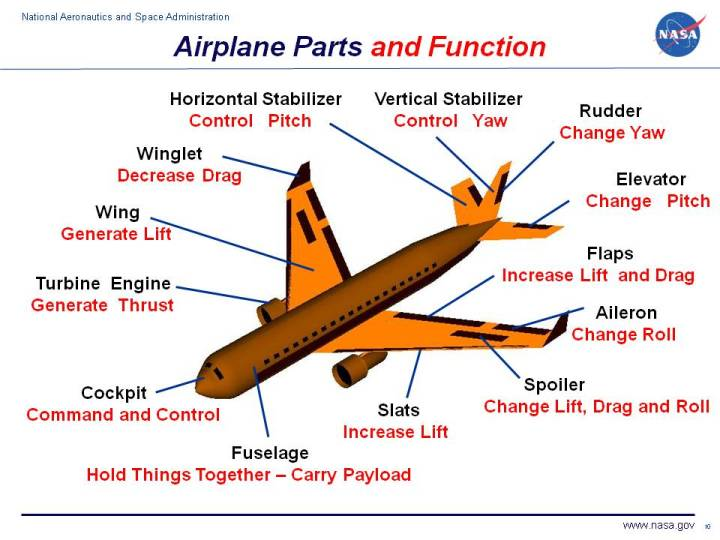
\includegraphics[scale=0.4]{parts}
\end{figure}

In a passenger jet, such as the B737, thrust is provided by the engine while other parts of the airplane control flight. As shown in Figure 3, the elevator can dynamically control pitch, while the horizontal stab statically controls pitch. Similarly, the vertical stab statically controls yaw while the rudder dynamically controls yaw. In wright stuff, there are no dynamically changing systems; therefore, it is imperative that the wing, rudder and horizontal stab are positioned correctly. The positioning of these will depend on the environment you fly in and other factors. 

The ideal turning radius is about 10 feet. You want the airplane to turn left, opposite to the rotation of the prop (Conservation of angular momentum). The plane also turns left because the wings are at an angle, providing a centripetal force. 

\begin{figure}[h]
\caption{An exaggerated rear view of a wing. Normally, angles are usually around 2-3$\degree$}
\centering
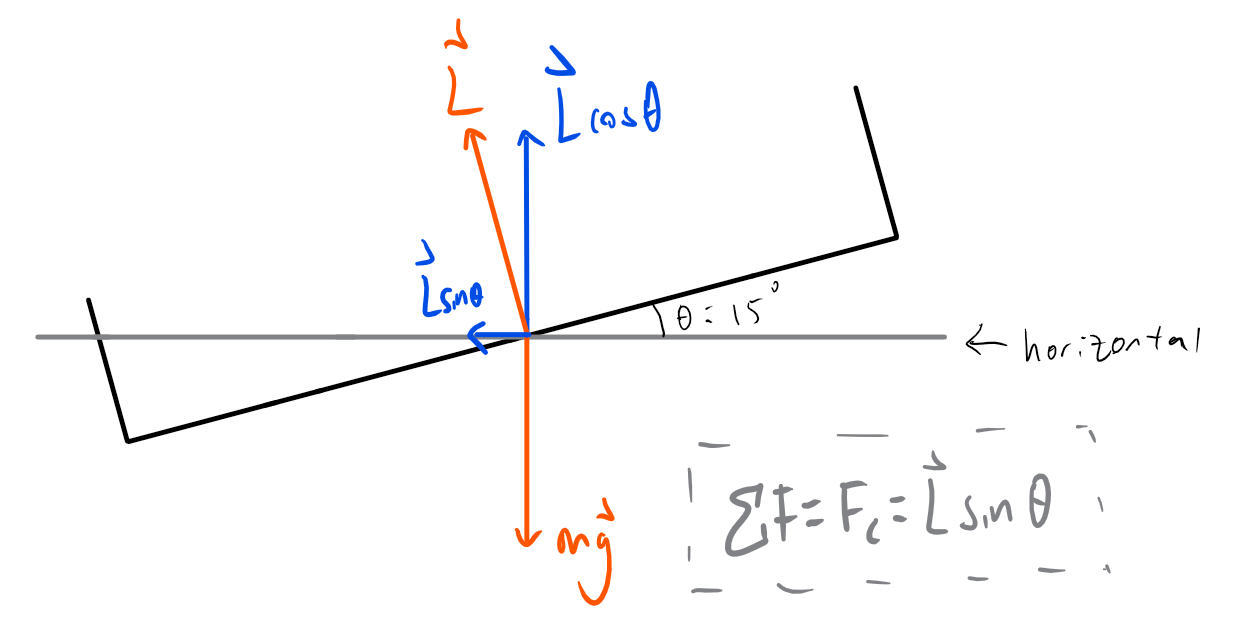
\includegraphics[scale=0.25]{wing}
\end{figure}

Once the horizontal angle of the wing is set, you can't adjust it. However, you can adjust the angle of the stab and the rudder. Rotating the rudder left or right will have the most effect at high speeds. To change the stab angle, sand the lower stab mount slightly. This is most effective at low speeds. 

At various different venues, air currents will become very significant, and you must adjust accordingly. With strong air currents, the airplane must be adjusted so that it will be stable. Do not fly first; watch other teams' planes and it will be visually apparent if the air currents are strong. In this case, move the CG forward and increase decalage. 

The key to success in Wright Stuff is a good pairing between rubber and propeller pitch. For rubber, start with 2 grams of medium-width .094" rubber, and move on from there. Thicker rubber provides more power and thrust but runs out quicker. This usually results in shorter flights. Remember to check how many winds you have left at landing. If you have a lot of rubber left, then you have a lot of unnecessary weight, and you can take some rubber out. If you are landing dead (no turns left), then you can add some more rubber. 

Propeller pitch is the angle that the prop makes in relation to its motion. It can be adjusted by bending the hub of the prop with pliers. Use a pitch guage to monitor the pitch and make sure that the two blades are even. Coarser pitch is best used with wide rubber, and fine pitch is better with thinner rubber. (Coarse=greater angle) The key to success is a good match between prop pitch and rubber. 

In rooms with low celings, you may want to try flaring props. They act as legal variable-pitch propellers. In the beginning, high-torque segment they flex out and use up the initial torque more quickly, and they return to normal during cruise and descent. These are useful in rooms with low celings because the plane will not climb as high. 

Another important part of propellers is sanding and trimming. Often, propellers will be too heavy and/or too large. You can trim them with some scissors, and sand with fine grit sandpaper. Try to keep the shape the same. There are instructions for this in the FF kit. Check the balance of the propeller by holding the shaft and letting it turn. If one side consistently goes to the bottom, you can add layers of scotch tape to the other side or sand down the heavy side. 

\end{document}